\documentclass[11pt,a4paper]{article}

\usepackage{amsmath}
\usepackage{fontspec}
\setmainfont{texgyrepagella}[
  Extension=.otf,
  UprightFont=*-regular,
  BoldFont=*-bold,
  ItalicFont=*-italic,
  BoldItalicFont=*-bolditalic
]
\usepackage[margin=2.15cm]{geometry}
\usepackage{microtype}
\usepackage{float}
\usepackage{graphicx}
\usepackage{booktabs}
\usepackage[font=small,labelfont=bf,skip=6pt]{caption}
\usepackage[hidelinks]{hyperref}
\usepackage{url}
\def\UrlBreaks{\do\/\do\-\do\:\do\.}

\setlength{\parskip}{0.35em}
\setlength{\parindent}{0pt}
\renewcommand{\arraystretch}{1.08}

\title{\textbf{CycleSense CPH}\\[0.35em]
\large Simulated-route coverage for bicycle counters\\ in central Copenhagen}
\author{[Group member names]}
\date{DTU 02807, Computational Tools for Data Science, Autumn 2026}

\begin{document}
\maketitle
\vspace{-1.6em}

\textbf{Summary.}
CycleSense asks where a limited number of counters on mapped Copenhagen streets would intercept simulated bicycle routes. Greedy maximum coverage is already a strong optimizer of that objective. At ten counters it covers 72.8\% of held-out uniform routes, against 40.4\% for a route-frequency ranking, and a mixed-integer solver certifies that the greedy calibration value is optimal at five and ten counters. At 10{,}000 routes, verified MinHash is about 8.3 times faster than streaming exact Jaccard. Louvain communities on this graph are fragmented, and balancing them does not raise held-out coverage. Placements move when the calibration sample or the route-choice rule changes, and published municipal bicycle counts rank only weakly with modeled traversal. The benchmark does not identify installation sites.

\section{Problem}

A counter records crossings of one street segment, and only a few segments can be instrumented. The questions are how close greedy coverage comes to a certified optimum, whether MinHash and locality-sensitive hashing preserve the Louvain partition and its counters, how far those counters move under new demand and route choice, and how they compare with published counting locations.

Two course methods are essential: MinHash with banding, and Louvain community detection. The method from outside the course is greedy maximization of a monotone submodular set function, checked against an exact mixed-integer linear program.

\section{Data}

The streets are OpenStreetMap, read from the BBBike Copenhagen extract with last-modified time 14 November 2026 and clipped with OSMnx~2.2 to longitudes 12.563--12.5965 and latitudes 55.6705--55.688 \cite{osm,bbbike,boeing}. The published graph has 1{,}157 routing nodes, 2{,}732 directed edges and 1{,}698 physical segments. A physical segment joins the two directions of one carriageway. Of these, 1{,}047 are eligible counter sites: at least 15 metres, and not rejected by the bicycle-access and service rules. The rule uses tags and length. It is not permission to install a counter. A later BBBike download can differ, and the PBF is not in Git. Reproduction uses the saved GraphML or the hashed file named in \texttt{docs/data\_sources.md} (Figure~\ref{fig:map}).

\begin{figure}[H]
  \centering
  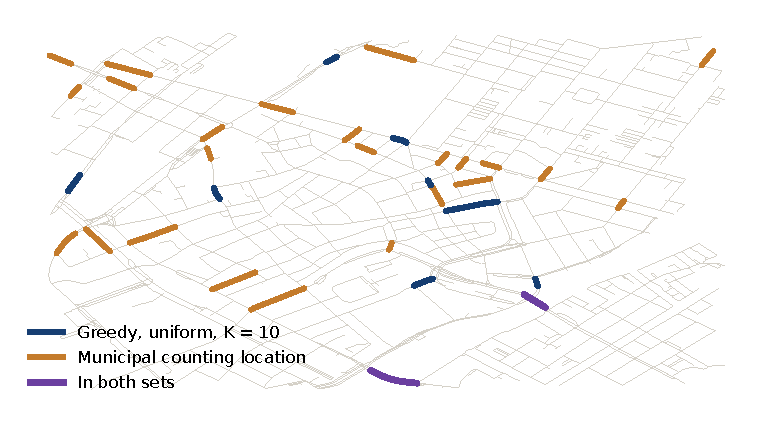
\includegraphics[width=0.72\textwidth]{figures/fig1_network.pdf}
  \caption{Indre By routing graph. Navy: uniform greedy set at \(K=10\). Orange: 26 name-verified municipal locations. Purple: a segment in both sets. Mapped streets, not observed trips.}
  \label{fig:map}
\end{figure}

Routes are shortest paths. Uniform routes draw both ends inside the rectangle. Commuter-proxy routes are biased toward a city-hall anchor. Each scenario has 500 calibration routes, seed 42, and 250 held-out routes, seed 10049. The splits do not share origin--destination pairs. Every accepted draw has weight 1, which is a sample weight and not a bicycle count. Counters are chosen on the calibration split only. The notebook is \texttt{notebooks/analysis.ipynb}; its tables are in \texttt{notebooks/assets/}.

Municipal bicycle figures come from Københavns Kommune's Trafiktal release, licence CC0, frozen on 21 November 2026 \cite{trafiktal}. Published bicycle AADT is the 07:00--19:00 count in both directions, multiplied by 1.03. It is not a continuous sensor reading. Inside the rectangle, 26 recurring counts match a physical segment by name. They are a counting programme, not a confirmed inventory of permanent sensors.

\section{Coverage and the algorithms}

Route \(r\) uses the physical-segment set \(E_r\). For a counter set \(S\) and nonnegative weights \(w_r\),
\begin{equation}
F(S)=\sum_{r} w_r\,\mathbf{1}(E_r\cap S\neq\emptyset), \qquad |S|\le K.
\label{eq:coverage}
\end{equation}
A route counts once. With nonnegative weights and only this cardinality constraint, \(F\) is monotone and submodular. The greedy rule adds the eligible segment of largest marginal gain and breaks ties by identifier. It reaches at least \(1-1/e\) of the optimal value of \(F\) on the routes used for selection \cite{nemhauser}. That guarantee is about the calibration objective. It does not transfer to held-out routes or to cyclists.

The same objective is the mixed-integer program
\begin{equation}
\begin{aligned}
\max \quad & \sum_{r} w_r y_r \\
\text{s.t.} \quad & \sum_{e} x_e \le K, \qquad
y_r \le \sum_{e\in E_r} x_e, \qquad
x_e,y_r\in\{0,1\}.
\end{aligned}
\label{eq:milp}
\end{equation}
SciPy passes the model to HiGHS. A run is optimal only when the solver says so, and held-out scores were not used to accept it.

Similarity treats each route as its set of physical-segment identifiers. Exact overlap is the Jaccard index \(J(A,B)=|A\cap B|/|A\cup B|\). MinHash replaces each set by a signature whose row-wise agreement estimates Jaccard \cite{broder}. Banding returns pairs that collide in a band. Those pairs are candidates. Exact Jaccard is then computed, and a pair is kept only when it meets the threshold 0.5. Graph-edge recall is the share of pairs above that threshold which the candidate list contains.

Routes are nodes of a similarity graph. Verified Jaccard similarity of at least 0.5 is a weighted edge, and isolated routes remain. Louvain partitions the graph \cite{blondel}. Partition agreement is the adjusted Rand index \cite{hubert}. The balanced placer keeps \(F\) and penalises unrepresented communities with \(\lambda=0.25\), fixed before the held-out comparison. \(\lambda=0\) is ordinary greedy.

\section{Optimization}

On uniform held-out routes at \(K=10\), greedy covers 72.8\%. Route frequency covers 40.4\%, geographic K-means 18.0\%, and one seeded random draw 6.4\%. On commuter-proxy routes greedy covers 69.2\%, and the order is the same (Figure~\ref{fig:baselines}).

\begin{figure}[H]
  \centering
  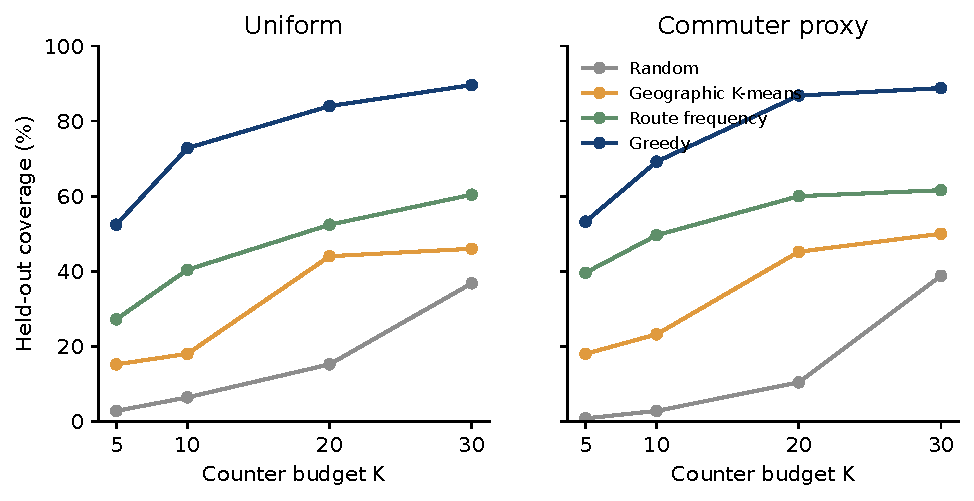
\includegraphics[width=\textwidth]{figures/fig2_baselines.pdf}
  \caption{Held-out modeled-route coverage. Random and geographic K-means use seed 42. Greedy and route frequency are deterministic.}
  \label{fig:baselines}
\end{figure}

Every saved unweighted HiGHS run returned status optimal. At \(K=5\) and \(K=10\), greedy matches the certified calibration value in both scenarios. At \(K=20\) the calibration gaps are 0.6 and 0.8 percentage points; at \(K=30\) they are 0.4 points. The certified set is not unique. Uniform \(K=10\) shares 8 of 10 segments between greedy and the solver. Both reach 74.0\% in calibration, while held-out coverage is 72.8\% for greedy and 68.8\% for the other set. On commuter-proxy routes the solver is ahead on the held-out sample, 70.4\% against 69.2\%. Held-out coverage can therefore fall when calibration coverage does not.

\section{Similarity, communities, and scale}

On the uniform calibration routes, 32 permutations and 16 bands of two rows miss one exact edge. Graph-edge recall is 0.998, and the adjusted Rand index against the exact Louvain partition is 0.97. An aggressive banding misses 458 edges and the index falls to 0.09, and the counters chosen from that partition change with it.

\begin{figure}[H]
  \centering
  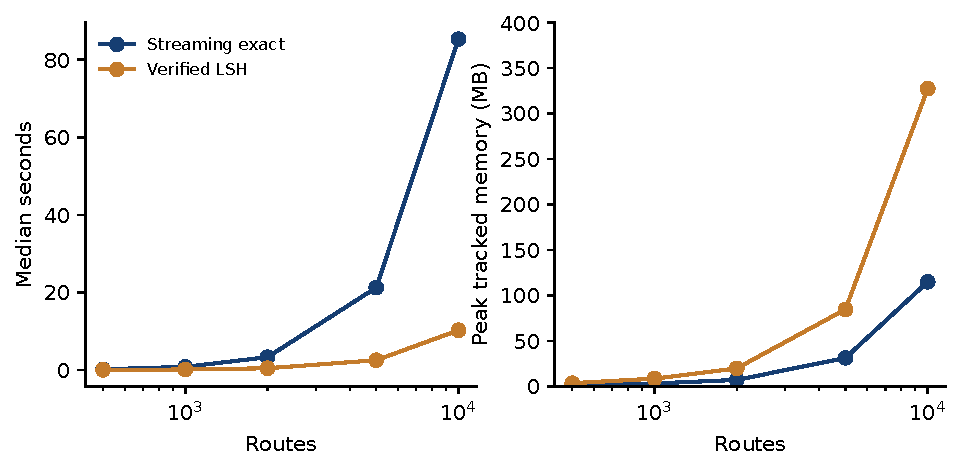
\includegraphics[width=\textwidth]{figures/fig3_lsh.pdf}
  \caption{Streaming exact Jaccard against verified hashing. Memory is peak Python-tracked allocation. The 10{,}000-route streaming time is one measurement; the hashed time is a median of three.}
  \label{fig:lsh}
\end{figure}

Figure~\ref{fig:lsh} compares pipelines that do not store the full pair matrix. At 10{,}000 routes, verified hashing takes 10.3 seconds and streaming exact Jaccard takes 85.3 seconds, about 8.3 times longer, in its one completed measurement. Peak tracked memory is 327~MB and 115~MB. The same memory ordering holds at 500 routes. At 10{,}000 routes, verifying candidates takes about 6.4 seconds and querying buckets about 1.0 second. These routes reuse one network.

At threshold 0.5 the uniform calibration graph yields 241 communities, 178 of them singletons, with modularity 0.91. The balanced placer at \(\lambda=0.25\) lowers held-out coverage from 72.8\% to 72.4\% on uniform routes and from 69.2\% to 66.8\% on commuter-proxy routes. Both lie inside the central 90\% of 30 label shuffles, so balancing does not consistently improve held-out coverage. The case \(\lambda=0\) reproduces the ordinary greedy edge set.

\section{When the routes change}

The saved counters were chosen on shortest paths. Each directed length was then multiplied by \(\exp(0.35Z)\), and a path was kept when its detour on the original lengths was at most 15\%. The counters were not refit. Over 20 seeds, mean coverage falls from 72.8\% to 65.7\% on uniform held-out routes and from 69.2\% to 65.9\% on commuter-proxy routes.

Training on the perturbed calibration routes does not close that gap. On fresh seeds, at the 15\% cap and \(K=10\), mean uniform coverage is 63.0\% for the route-choice placer and 64.1\% for pooled shortest-path greedy. The commuter-proxy means are 64.2\% and 63.2\%. The route-choice objective has no consistent gain.

A new calibration sample moves the streets more than the coverage. Across 30 uniform draws, greedy at \(K=10\) uses 61 distinct segments. Mean pairwise Jaccard similarity of the sets is 0.27. Held-out coverage stays between 65.6\% and 73.6\%. Only Knippelsbro\,/\,Børsgade appears in every uniform draw and in every commuter-proxy draw (Figure~\ref{fig:stability}). A repeated street name is a different segment. The frequencies describe this sampler. They are not installation probabilities.

\begin{figure}[H]
  \centering
  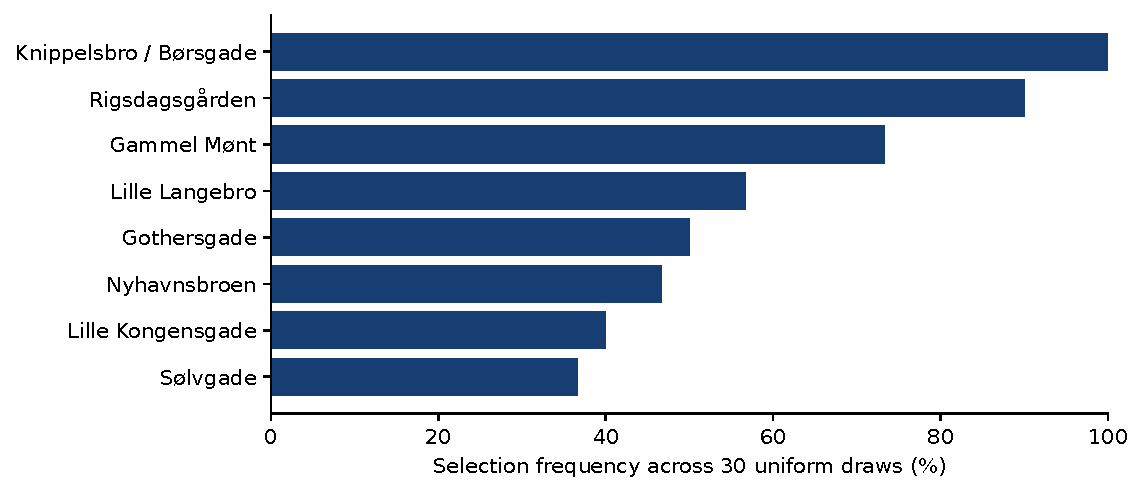
\includegraphics[width=0.92\textwidth]{figures/fig4_stability.pdf}
  \caption{Uniform greedy at \(K=10\): selection frequency over 30 calibration draws of 500 routes. Each bar is one physical segment.}
  \label{fig:stability}
\end{figure}

\section{Published counts and mapped facilities}

The 26 name-verified sites cover 73.6\% of uniform held-out routes and 72.4\% of commuter-proxy held-out routes. Five greedy segments chosen on the calibration routes raise those figures to 83.6\% and 82.8\%. Ten segments raise them to 87.2\% and 85.2\% (Figure~\ref{fig:municipal}). The increase is simulated-route coverage.

\begin{figure}[H]
  \centering
  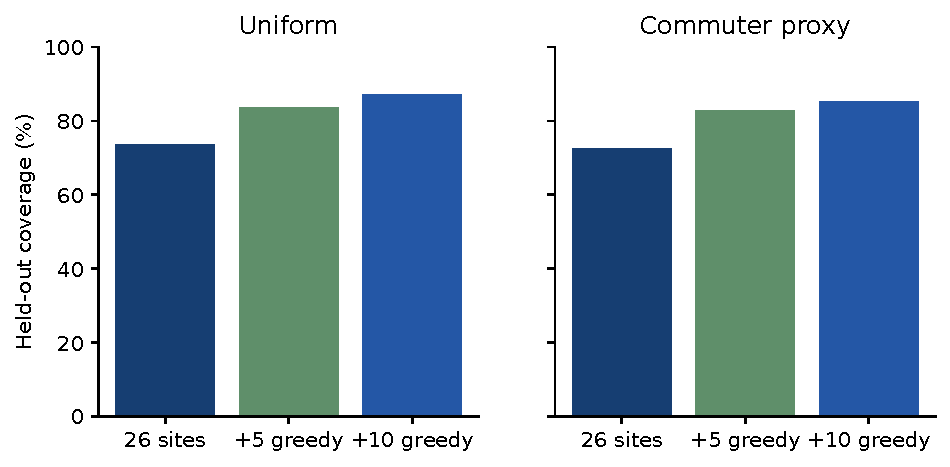
\includegraphics[width=\textwidth]{figures/fig5_municipal.pdf}
  \caption{Held-out coverage of the 26 published locations and of those locations plus greedy segments. The scale is the share of simulated routes.}
  \label{fig:municipal}
\end{figure}

Spearman correlation between published bicycle AADT and modeled traversal is 0.26 on the uniform calibration routes, with a permutation \(p\)-value of 0.21 from 2{,}000 draws. Unique coverage and equal-share attribution agree no more closely. Dronning Louises Bro, on the west edge of the rectangle, has AADT 33{,}000 and no simulated traversal: the sampled trips start and end inside the clipped graph.

Keeping only segments tagged as dedicated cycleways leaves 107 of 1{,}047 candidates and lowers uniform held-out coverage at \(K=10\) from 72.8\% to 30.0\%. A missing cycleway tag is not evidence that a facility is absent. On the uniform calibration routes, Knippelsbro uniquely covers 7.4 percentage points, while an equal share of each municipal site on a covered route assigns it 12.9 points. Those shares sum to the coverage of all 26 sites. Shared modeled coverage is not a case for removing a counting site.

\section{What the results establish}

Greedy meets the certified calibration value of \(F\) at \(K=5\) and \(K=10\), and the later gaps stay below one percentage point, against a generic guarantee near 63\%. The binding limits are elsewhere: simulated shortest paths, sets that move while coverage does not, a hashing method that trades memory for speed, and a weak link to published counts.

The supported claim is about this simulation: greedy coverage is strong and often certified, and the selected set is less stable than its coverage. It does not locate real installations.

\begin{thebibliography}{9}
\bibitem{osm} OpenStreetMap contributors. OpenStreetMap. \url{https://www.openstreetmap.org}. Data under the Open Database Licence.
\bibitem{bbbike} BBBike. Copenhagen OpenStreetMap extract, last-modified 14 November 2026. \url{https://download.bbbike.org/osm/bbbike/Copenhagen/Copenhagen.osm.pbf}. Living file. Hash in \texttt{docs/data\_sources.md}.
\bibitem{boeing} Boeing, G. (2017). OSMnx: New methods for acquiring, constructing, analyzing, and visualizing complex street networks. \emph{Computers, Environment and Urban Systems}, 65, 126--139.
\bibitem{trafiktal} Københavns Kommune, Bydata. Trafiktal. \url{https://www.opendata.dk/city-of-copenhagen/trafiktal}. CC0. Snapshot frozen 21 November 2026.
\bibitem{nemhauser} Nemhauser, G.~L., Wolsey, L.~A., and Fisher, M.~L. (1978). An analysis of approximations for maximizing submodular set functions---I. \emph{Mathematical Programming}, 14, 265--294.
\bibitem{broder} Broder, A.~Z. (1997). On the resemblance and containment of documents. \emph{Proceedings of the Compression and Complexity of Sequences 1997}, 21--29.
\bibitem{blondel} Blondel, V.~D., Guillaume, J.-L., Lambiotte, R., and Lefebvre, E. (2008). Fast unfolding of communities in large networks. \emph{Journal of Statistical Mechanics: Theory and Experiment}, P10008.
\bibitem{hubert} Hubert, L. and Arabie, P. (1985). Comparing partitions. \emph{Journal of Classification}, 2, 193--218.
\end{thebibliography}

\section*{Appendix. Group contributions}
Individual contributions and the group size are not recorded in the repository. Replace this note, before upload, with one line per member: name and contribution. The limit used here is 11{,}000 characters excluding white space. A group of five may use 12{,}500.

\end{document}
